% The column generation benchmark runner: what it is, why, and what comes next. For the colleagues.
% Build: latexmk -pdf slides.tex
\documentclass[aspectratio=169]{beamer}

\usetheme{Boadilla}
\usecolortheme{default}

\usepackage[T1]{fontenc}
\usepackage[utf8]{inputenc}
\usepackage{booktabs}
\usepackage{array}
\usepackage{listings}
\usepackage{tikz}
\usetikzlibrary{positioning,arrows.meta,fit}

\definecolor{GLBlue}{RGB}{22,63,95}
\definecolor{GLGray}{RGB}{96,104,114}
\definecolor{GLLight}{RGB}{232,240,248}
\definecolor{GLOrange}{RGB}{214,110,30}
\definecolor{GLRed}{RGB}{190,40,40}

\setbeamercolor{normal text}{fg=black,bg=white}
\setbeamercolor{title}{fg=GLBlue}
\setbeamercolor{subtitle}{fg=GLGray}
\setbeamercolor{frametitle}{fg=GLBlue,bg=GLBlue!6}
\setbeamercolor{titlelike}{fg=GLBlue}
\setbeamercolor{author}{fg=GLGray}
\setbeamercolor{date}{fg=GLGray}
\setbeamercolor{structure}{fg=GLBlue}
\setbeamercolor{itemize item}{fg=GLBlue}
\setbeamercolor{itemize subitem}{fg=GLGray}
\setbeamercolor{block title}{fg=white,bg=GLBlue}
\setbeamercolor{block body}{fg=black,bg=GLLight}

\setbeamerfont{title}{size=\LARGE,series=\bfseries}
\setbeamerfont{subtitle}{size=\normalsize}
\setbeamerfont{frametitle}{size=\Large,series=\bfseries}

\setbeamertemplate{navigation symbols}{}
\setbeamertemplate{headline}{}
\setbeamertemplate{footline}[frame number]
\setbeamertemplate{itemize subitem}[triangle]

\lstset{
  basicstyle=\ttfamily\scriptsize,
  keywordstyle=\color{GLBlue}\bfseries,
  commentstyle=\color{GLGray}\itshape,
  stringstyle=\color{GLBlue!70!black},
  backgroundcolor=\color{GLLight},
  frame=single,
  rulecolor=\color{GLBlue},
  columns=fullflexible,
  keepspaces=true,
  showstringspaces=false,
  xleftmargin=4pt,
  xrightmargin=4pt,
}
\lstdefinelanguage{toml}{
  morecomment=[l]{\#},
  morestring=[b]",
  sensitive=true,
}

\tikzset{
  box/.style={draw=GLBlue, fill=GLLight, rounded corners=2pt, align=center, font=\small,
    minimum height=2.2em, inner sep=4pt},
  later/.style={box, dashed, draw=GLGray, fill=white, text=GLGray},
  file/.style={draw=GLGray, fill=white, align=left, font=\scriptsize\ttfamily, inner sep=3pt},
  flow/.style={-{Stealth[length=5pt]}, GLBlue, thick},
}

\title{A benchmark runner for column generation}
\subtitle{One maintained tool to measure every rcspp feature}
\author{Leo Marbehan}
\date{November 2026}

\begin{document}

\begin{frame}[plain]
  \titlepage
\end{frame}

%--------------------------------------------------------------
\begin{frame}{Where the repository stands}
  \begin{columns}[T]
    \begin{column}{0.5\textwidth}
      \textbf{Shipped: \texttt{rcspp.column\_generation}}, pure Python
      \begin{itemize}\small
        \item master problem over \texttt{highspy} or \texttt{gurobipy}
        \item graph pricer over the C++ RCSPP search, pricing stages
        \item the loop, starts, tolerances, statistics
        \item a documentation page with a tested example
      \end{itemize}
    \end{column}
    \begin{column}{0.46\textwidth}
      \textbf{Kept as an example}: the C++ layer
      \begin{itemize}\small
        \item \texttt{examples/column\_generation}, off by default
        \item its Python bindings, compiled in only when asked
        \item nothing shipped depends on it
      \end{itemize}
    \end{column}
  \end{columns}

  \vspace{0.6em}
  \begin{itemize}\small
    \item Eight pull requests in review, merged together; CI passes on the last one.
    \item Python only, decided after the full comparison of the two layers: 1,204 runs, \textbf{same results
      everywhere}, same speed within the run-to-run noise on realistic runs.
  \end{itemize}
\end{frame}

%--------------------------------------------------------------
\begin{frame}{What we want, and why}
  \textbf{Today}: the measurements are throwaway scripts on a side branch.
  \begin{itemize}\small
    \item settings through environment variables, a hard-coded list of configurations
    \item the code measured is whatever a checkout next to the scripts holds: \textbf{not recorded}
    \item every next task (ported examples, ng-routes, the bidirectional search, \ldots) would write its own
      one-off comparison
  \end{itemize}

  \vspace{0.4em}
  \begin{block}{What we want}
    \begin{itemize}\small
      \item \textbf{one maintained tool} in the repository, next to the code it measures
      \item every rcspp feature behind a simple parameter, no code to change
      \item \textbf{reproducible}: each run records its code, versions and machine, and can be rerun as is
      \item readable: a new user finds in it how to run column generation
    \end{itemize}
  \end{block}
\end{frame}

%--------------------------------------------------------------
\begin{frame}{The proposal at a glance}
  \centering
  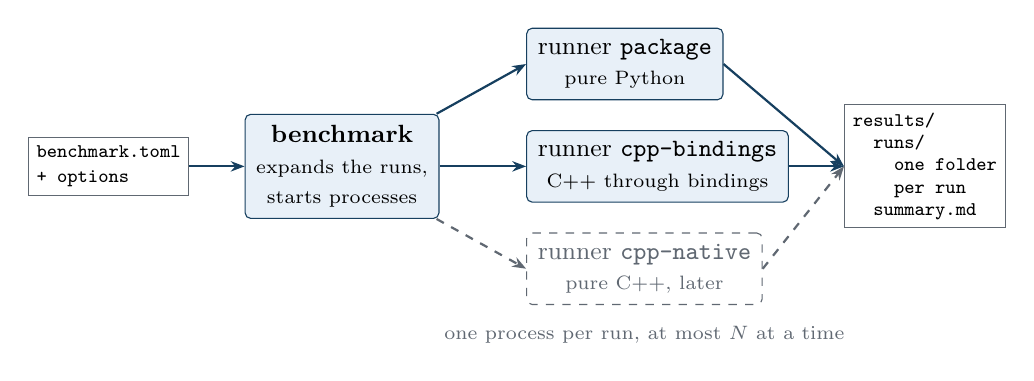
\begin{tikzpicture}[node distance=0.5cm and 0.7cm]
    \node[file] (input) {benchmark.toml\\[1pt]+ options};
    \node[box, right=of input] (bench) {\textbf{benchmark}\\\scriptsize expands the runs,\\
      \scriptsize starts processes};
    \node[box, right=1.1cm of bench, yshift=1.3cm] (package) {runner \texttt{package}\\\scriptsize pure Python};
    \node[box, right=1.1cm of bench] (cppex) {runner \texttt{cpp-bindings}\\\scriptsize C++ through bindings};
    \node[later, right=1.1cm of bench, yshift=-1.3cm] (cppprog) {runner \texttt{cpp-native}\\
      \scriptsize pure C++, later};
    \node[file, right=of cppex] (runs) {results/\\\ \ runs/\\\ \ \ \ one folder\\\ \ \ \ per run\\
      \ \ summary.md};
    \draw[flow] (input) -- (bench);
    \draw[flow] (bench) -- (package.west);
    \draw[flow] (bench) -- (cppex.west);
    \draw[flow, dashed, GLGray] (bench) -- (cppprog.west);
    \draw[flow] (package.east) -- (runs.west);
    \draw[flow] (cppex.east) -- (runs.west);
    \draw[flow, dashed, GLGray] (cppprog.east) -- (runs.west);
    \node[font=\scriptsize, text=GLGray, below=0.15cm of cppprog] {one process per run, at most $N$ at a time};
  \end{tikzpicture}

  \vspace{0.6em}
  \raggedright\small
  \begin{itemize}
    \item \textbf{Runners}: one per layer, each does one run and can be called alone.
    \item \textbf{Benchmark}: takes one or more runs and calls the runners through a fixed contract
      (options in, a run folder out). It never imports them, so a C++ program fits the same way.
  \end{itemize}
\end{frame}

%--------------------------------------------------------------
\begin{frame}[fragile]{The runners}
  \begin{columns}[T]
    \begin{column}{0.42\textwidth}
      \begin{itemize}\small
        \item \texttt{package}: the shipped Python package
        \item \texttt{cpp-bindings}: the C++ example layer, through its bindings
        \item \texttt{cpp-native}: pure C++, no Python (later)
      \end{itemize}

      \vspace{0.3em}
      \begin{itemize}\footnotesize
        \item the body of a runner is \textbf{the column generation calls}, about 100 lines: also the example a
          new user reads
        \item options, instances, records and output are \textbf{shared}, never duplicated
        \item a test checks that every runner gives the same LP value, iterations and columns
      \end{itemize}
    \end{column}
    \begin{column}{0.55\textwidth}
      \small The body of the \texttt{package} runner (sketch):
\begin{lstlisting}[language=Python, basicstyle=\ttfamily\tiny]
import rcspp.column_generation as cg

master = cg.MasterProblem(cg.HighspyMasterSolver(model))
stages = [cg.PricingStage(s.algorithm, s.parameters)
          for s in options.pricing.stages]
pricer = master.add_pricer(
    cg.GraphPricer(instance.graph(), stages),
    cg.ConvexityRow())
instance.add_start(master, pricer, options.start)
result = cg.ColumnGeneration(master, parameters).run()
write_result(output, result)   # result.json
\end{lstlisting}
    \end{column}
  \end{columns}
\end{frame}

%--------------------------------------------------------------
\begin{frame}{The benchmark}
  \begin{itemize}
    \item One or more runs; \textbf{one run is just a runner call}, so the same tool serves for a quick check.
    \item A \textbf{matrix} is a product of option lists: instances $\times$ runners $\times$ masters $\times$
      pricing $\times$ \ldots, plus any extra runs.
    \item \textbf{Processes}: at most $N$ runs at a time, 1 by default.
      \begin{itemize}\small
        \item parallel runs disturb each other's timings: recorded, and flagged in the summary
        \item Gurobi limited to one thread then
      \end{itemize}
    \item \textbf{Repeats as rounds}: every run once, then again; slow changes of the machine (heat, a background
      job) spread over every case instead of one.
    \item \textbf{Resumable}: a finished run is skipped; a \texttt{STOP} file stops after the runs in progress;
      a timeout kills a stuck run.
    \item Refuses to mix results from different code, solver versions or machines in one folder.
  \end{itemize}
\end{frame}

%--------------------------------------------------------------
\begin{frame}[fragile]{Inputs: options and TOML files}
  \begin{columns}[T]
    \begin{column}{0.42\textwidth}
      \begin{itemize}\small
        \item every option has \textbf{one name}: \texttt{-{}-master gurobipy} on the command line, or
          \texttt{master = "gurobipy"} in a file; the command line wins
        \item every building block is a table: a \texttt{type} and its parameters
        \item any block can be \textbf{named and reused}; the built-in presets are a TOML file of the same
          format
        \item pricing is a list of stages, each an algorithm and its search parameters
        \item unknown keys are refused before the first run
      \end{itemize}
    \end{column}
    \begin{column}{0.55\textwidth}
\begin{lstlisting}[language=toml]
[benchmark]
processes = 1
repeats = 3

[pricing.heuristics-first]
stages = [
  { algorithm = "greedy", max_solutions = 100 },
  { algorithm = "tabu", max_solutions = 20,
    max_iterations = 1000 },
  { algorithm = "simple" },
]

[defaults]
start = { type = "single-customer" }

[matrix]             # the product of these lists
instance = ["C101_25", "R201_25"]
layer = ["package", "cpp-bindings"]
master = ["highspy", "gurobipy"]
pricing = ["exact", "heuristics-first"]
\end{lstlisting}
    \end{column}
  \end{columns}
\end{frame}

%--------------------------------------------------------------
\begin{frame}[fragile]{Outputs: one folder per run}
  \begin{columns}[T]
    \begin{column}{0.5\textwidth}
\begin{lstlisting}
results/
  benchmark.toml   the input, expanded
  metadata.json    processes, runs, machine, ...
  summary.md, summary.csv
  status.txt       the runs in progress
  runs/
    R201_25-package-highspy-tabu-r2/
      run.toml       the run's own options
      command.txt    the exact command line
      metadata.json  start, end, load, ...
      result.json    the results
      log.txt
\end{lstlisting}
    \end{column}
    \begin{column}{0.46\textwidth}
      \begin{itemize}\small
        \item \texttt{result.json}: status, LP value, iterations, columns, master, pricing and total seconds,
          plus what the statistics add
        \item \textbf{rerun as is}: \texttt{run.toml} holds the expanded values, not preset names, so it runs
          the same after a preset changes
        \item \textbf{summary}: per case the median, minimum, maximum and spread over the rounds; two runners
          compared with our equivalence rule
      \end{itemize}
    \end{column}
  \end{columns}
\end{frame}

%--------------------------------------------------------------
\begin{frame}{What each run records, and statistics}
  \begin{columns}[T]
    \begin{column}{0.5\textwidth}
      \textbf{Recorded with every run}
      \begin{itemize}\small
        \item the source: commit, uncommitted changes, branch
        \item the build: configuration and compiler
        \item versions: Python, rcspp, numpy, HiGHS, Gurobi
        \item the machine: a label, OS, CPU, cores, memory
        \item the load during the run: other processes' CPU, memory, CPU frequency, on battery or not
      \end{itemize}
    \end{column}
    \begin{column}{0.46\textwidth}
      \textbf{Statistics: one collector each}
      \begin{itemize}\small
        \item a name, its cost, an option turning it on
        \item now: times, peak memory, processor time, the summary's figures
        \item added when a task needs them: per-iteration values, the time split per iteration, per-stage counts,
          the Lagrangian bound
      \end{itemize}
    \end{column}
  \end{columns}

  \vspace{0.6em}
  \begin{block}{Why}
    \small A result without its code, versions and machine cannot be compared with the next one.
  \end{block}
\end{frame}

%--------------------------------------------------------------
\begin{frame}{Where it is}
  \begin{itemize}
    \item \textbf{Design decided}; a pull request on top of the column generation stack.
    \item \textbf{Done}: the folder and its README, options and TOML files, instances (Solomon VRPTW), run folders
      and records; 68 tests, run in CI.
    \item \textbf{Next}: the two runners, the benchmark, the summary, a benchmark file reproducing the full
      comparison.
  \end{itemize}

  \vspace{0.6em}
  \textbf{Instances}: one small interface (read, build the graph and rows, give starting columns),
  Solomon VRPTW for now, with the \emph{one route per customer} start. Other instance types can plug in later
  without changing the format.
\end{frame}

%--------------------------------------------------------------
\begin{frame}{Next: the rest of the first phase}
  Each task adds \textbf{its option to the runner} instead of its own script.

  \vspace{0.4em}
  \small
  \begin{tabular}{@{}>{\raggedright\arraybackslash}p{0.36\textwidth}>{\raggedright\arraybackslash}p{0.58\textwidth}@{}}
    \toprule
    task & what it adds \\
    \midrule
    Python VRP example on the package & the example rewritten on the package, its own master dropped \\
    C++ VRP example on the C++ example layer & runner \texttt{cpp-native}: pure C++, a third measure \\
    ng-routes & an ng size option for the graph \\
    the engine's newer features & the bidirectional search and its options, as stage parameters \\
    many cheap iterations & truncated pricing presets; the three runners compared \\
    \bottomrule
  \end{tabular}

  \vspace{0.6em}
  \begin{itemize}\small
    \item then: the stack merged; the API reference of the package in the documentation
    \item then: re-scoping the next phases for the Python package, including several vehicle types
  \end{itemize}
\end{frame}

%--------------------------------------------------------------
\begin{frame}{Then: the second phase, performance}
  Planned, to be re-scoped for the Python package; each measured with the runner.
  \begin{itemize}\small
    \item \textbf{pricing strategies}: stages with budgets that grow, several pricers
    \item \textbf{a column pool} in the loop: price stored columns first, column management
    \item \textbf{a Lagrangian bound}, and an early stop on a gap or a cutoff
    \item \textbf{stabilization} (smoothing of the duals)
    \item \textbf{statistics and records}: the levels, standard log columns, hooks; the runner's records
    \item parallel pricers (optional)
  \end{itemize}

  \vspace{0.4em}
  \small\textcolor{GLGray}{Later phases, designed but not decided: branch-and-price; SoPlex and SCIP.}
\end{frame}

%--------------------------------------------------------------
\begin{frame}{Longer term}
  \begin{columns}[T]
    \begin{column}{0.32\textwidth}
      \textbf{Regression tests}
      \begin{itemize}\small
        \item a fixed benchmark file
        \item results must not change: LP value, iterations, columns
        \item times compared with the last recorded run, on a quiet machine
        \item a small run in CI
      \end{itemize}
    \end{column}
    \begin{column}{0.32\textwidth}
      \textbf{Precise benchmarks on Compute Canada}
      \begin{itemize}\small
        \item cluster jobs on dedicated nodes: little noise, many repeats
        \item the same runners and files; results carry their machine
        \item larger instances and longer limits
      \end{itemize}
    \end{column}
    \begin{column}{0.32\textwidth}
      \textbf{Comparison with other solvers}
      \begin{itemize}\small
        \item any program that follows the contract is a runner
        \item other RCSPP and column generation codes measured on the same instances, in the same format
      \end{itemize}
    \end{column}
  \end{columns}
\end{frame}

%--------------------------------------------------------------
\begin{frame}{Feedback welcome}
  \begin{itemize}
    \item Which instances and cases should the regression benchmark hold?
    \item Which other solvers would be worth a runner?
    \item Compute Canada: which allocation and cluster to use?
    \item Anything a run should record that is missing?
  \end{itemize}
\end{frame}

\end{document}
